\chapter{Configuración y resultados del entrenamiento final}
\label{cap:AnexoH}

Este anexo documenta los hiperparámetros del modelo desplegado en producción y los resultados de evaluación obtenidos en los conjuntos de validación y prueba de CodiEsp~\cite{miranda2020}.

\section{Modelo base}

Se emplea \texttt{IIC/RigoBERTa-Clinical}~\cite{garciasubies2026rigobertaclinical}, variante clínica de RigoBERTa~\cite{vacaserrano2022rigoberta} basada en la arquitectura XLM-RoBERTa-large. La ventana de contexto nativa del modelo es de 512 \emph{tokens}, que es también la longitud máxima empleada en entrenamiento e inferencia.

\section{Hiperparámetros}

La Tabla~\ref{tab:hyperparams} recoge la configuración de la ejecución de producción (\texttt{20260530T030233Z}, paso~36).

\begin{table}[h]
\centering
\caption{Hiperparámetros del entrenamiento final.}
\label{tab:hyperparams}
\begin{tabular}{lll}
\hline
\textbf{Parámetro} & \textbf{Valor} & \textbf{Descripción} \\
\hline
\multicolumn{3}{l}{\textit{Datos}} \\
\texttt{num\_codes}      & 1767          & Clases (códigos CIE-10 completos presentes en CodiEsp) \\
\texttt{max\_length}     & 512           & Longitud máxima de secuencia en \emph{tokens} \\
\texttt{full\_codes}     & \texttt{True} & Granularidad completa (p.\,ej.\ \texttt{E11.9}), sin truncar a 3~caracteres \\
\hline
\multicolumn{3}{l}{\textit{Optimización}} \\
\texttt{lr}              & $10^{-4}$     & Tasa de aprendizaje \\
\texttt{warmup\_ratio}   & 0{,}1         & Fracción de pasos de calentamiento \\
\texttt{lr\_schedule}    & plateau       & Reducción al detectar estancamiento en val. F1 \\
\texttt{weight\_decay}   & 0{,}1         & Regularización L2 \\
\texttt{epochs\_max}     & 150           & Máximo de épocas permitido \\
\texttt{epochs\_run}     & 150           & Épocas ejecutadas (alcanzó el máximo sin parada temprana) \\
\texttt{patience}        & 20            & Épocas sin mejora antes de parar \\
\hline
\multicolumn{3}{l}{\textit{Arquitectura}} \\
\texttt{dropout}         & 0{,}3         & \emph{Dropout} en la cabeza de clasificación \\
\texttt{freeze\_layers}  & 20            & Capas del \emph{encoder} congeladas al inicio \\
\texttt{unfreeze\_every} & 30            & Épocas entre descongelaciones \\
\texttt{unfreeze\_layers}& 4             & Capas descongeladas en cada paso \\
\texttt{unfreeze\_lr\_ratio} & 0{,}1     & Factor de reducción de LR para capas descongeladas \\
\hline
\multicolumn{3}{l}{\textit{Función de pérdida}} \\
\texttt{label\_smoothing} & 0{,}1       & Suavizado de etiquetas \\
\texttt{pos\_weight\_cap} & 10{,}0      & Peso máximo de la clase positiva (desequilibrio) \\
\hline
\multicolumn{3}{l}{\textit{Batch}} \\
\texttt{batch\_size}     & 8             & Tamaño de mini-lote efectivo en GPU \\
\texttt{grad\_accum}     & 4             & Pasos de acumulación de gradiente \\
\texttt{effective\_batch}& 32            & Tamaño de lote efectivo resultante \\
\hline
\multicolumn{3}{l}{\textit{Inferencia}} \\
\texttt{threshold}       & 0{,}3         & Umbral de probabilidad para activar una etiqueta \\
\texttt{pretrain\_epochs}& 10            & Épocas de precalentamiento con todo congelado \\
\texttt{attn\_impl}     & \texttt{flash\_attention\_2} & Implementación de atención (FlashAttention 2) \\
\hline
\end{tabular}
\end{table}

\section{Resultados de evaluación}

El sistema emplea dos estrategias de umbral diferentes. Durante el entrenamiento se usa un umbral global fijo para monitorizar la mejora. También se evaluaron umbrales por clase optimizados sobre el conjunto de validación, que ajustan individualmente el punto de corte de cada uno de los 1.767 códigos; se descartaron para producción por sobreajustar la validación (véase más abajo).

La Tabla~\ref{tab:final-results} muestra ambas métricas para el modelo de producción (ejecución \texttt{20260530T030233Z}, paso~36).

\begin{table}[h]
\centering
\caption{Resultados del modelo final (paso~36) en validación y prueba, por estrategia de umbral. Generada con \texttt{make ai-eval-test} (\texttt{ai\_engine/eval\_test.py}); los valores quedan en \texttt{model/eval\_test.json}.}
\label{tab:final-results}
\begin{tabular}{llrrl}
\hline
\textbf{Conjunto} & \textbf{Umbral} & \textbf{F1-micro} & \textbf{F1-macro} & \textbf{MAP} \\
\hline
Validación & global 0,2 & 0{,}4861 & 0{,}106 & 0{,}558$^{r}$ \\
Test       & global 0,2 & 0{,}4946 & 0{,}108 & \textbf{0{,}454}$^{g}$ / 0{,}555$^{r}$ \\
Test       & por clase  & 0{,}485  & 0{,}112 & n/d \\
\hline
\end{tabular}

\smallskip\par\footnotesize $^{g}$~MAP sobre el gold completo (directamente comparable con el \emph{benchmark} CodiEsp). $^{r}$~MAP restringido a los 1.767 códigos del vocabulario del modelo. Los umbrales por clase se ajustan sobre validación y no mejoran al global (F1-micro 0,485 frente a 0,495 en prueba), por lo que la configuración desplegada emplea el umbral global de 0,2.
\end{table}

La ejecución desplegada es \texttt{20260921T091919Z}, la de pérdida de ordenación descrita en la subsección~\ref{sec:anexoF-alineacion}, publicada en Hugging Face como \texttt{zlpr-map}. Con umbral global de 0,2 alcanza F1-micro = 0{,}4861 en validación y 0{,}4946 en prueba. El MAP no aparece para los umbrales por clase porque no depende del umbral: es una métrica de ordenación y sería el mismo valor repetido. Los umbrales por clase, ajustados sobre validación, no compensan: se quedan en 0,485 en prueba frente a los 0,495 del umbral global, de modo que se emplea este último. El MAP por documento sobre el conjunto de prueba (métrica oficial del \emph{benchmark} CodiEsp) es \textbf{0{,}454} sobre el gold completo (0{,}555 restringido al vocabulario del modelo), situándose dentro del rango del \emph{benchmark}~\cite{miranda2020}, por detrás de los \emph{ensembles} y diccionarios de las primeras posiciones. El \emph{recall} de 0,459 debe leerse contra el techo de 0,825 que impone el vocabulario del modelo (497 de los 2.842 pares del \emph{gold} de prueba son códigos que no aparecen en entrenamiento): supone el 55,7\,\% del máximo alcanzable.

\section{Selección del modelo desplegado}
\label{sec:anexoH-candidatos}

La elección no se hizo por la mejor cifra de validación sino midiendo en prueba a todos los candidatos, porque la ordenación por validación no se transfiere: \texttt{c102909} tenía el mejor F1 de validación de toda la serie (0,5028) y en prueba queda por debajo del modelo al que sustituía en esa misma métrica. La Tabla~\ref{tab:candidatos} recoge la comparación, generada con \texttt{make ai-eval-candidatos} y \texttt{make ai-eval-candidatos-fusion} (\texttt{ai\_engine/eval\_test.py}, \texttt{rerank\_map.py} y \texttt{tabla\_candidatos.py}).

\begin{table}[h]
\centering
\small
\caption{Candidatos a despliegue, medidos sobre el conjunto de prueba. El MAP fusionado corresponde al motor \texttt{engine=fused}, con $\beta$ elegido en validación para cada modelo. La fila resaltada es el modelo desplegado.}
\label{tab:candidatos}
\begin{tabular}{llrrr}
\hline
\textbf{Modelo} & \textbf{Diferencia} & \textbf{MAP} & \textbf{MAP fusión} & \textbf{F1-micro} \\
\hline
\rowcolor{gray!15}
\textbf{zlpr-map} & Pérdida ZLPR, checkpoint elegido por MAP & \textbf{0{,}454} & \textbf{0{,}553} & \textbf{0{,}495} \\
c102909 & Mejor F1 de validación de la serie (0,503) & 0{,}444 & 0{,}547 & 0{,}482 \\
Paso 36 & Modelo desplegado hasta esta selección & 0{,}437 & 0{,}545 & 0{,}489 \\
c225633 & Variante descartada de la misma serie & 0{,}433 & n/d & 0{,}480 \\
\hline
\end{tabular}

\vspace{2mm}
{\footnotesize El modelo desplegado gana en las tres métricas, que es la condición que se impuso para promocionarlo: una mejora de MAP a costa del F1 habría mejorado un titular y empeorado otro. La fila \texttt{c225633} se conserva porque justifica su descarte; su checkpoint se borró tras medirlo y su MAP fusionado no llegó a calcularse.}
\end{table}

\paragraph{Procedencia de las cifras.} Las métricas de esta tabla proceden de dos pasadas de evaluación distintas: el barrido de umbral y el MAP de prueba se calculan con \texttt{eval\_test.py}, mientras que las cifras de validación reportadas como referencia del paso~36 provienen del registro de entrenamiento. Ambas difieren en la tercera cifra decimal (por ejemplo, MAP de prueba 0,4539 frente a 0,4535) porque la inferencia de una de ellas se realiza con precisión reducida. La diferencia no altera ninguna conclusión, pero conviene declararla para que el lector no la interprete como una inconsistencia.

La diferencia entre F1-micro y F1-macro refleja el fuerte desequilibrio de clases del corpus: el modelo rinde bien sobre los códigos frecuentes, pero tiene dificultades con los poco representados. Este es un límite inherente al corpus de entrenamiento de 500 documentos, donde la mayoría de los 1.767 códigos aparecen menos de cinco veces.

\section{Curvas de entrenamiento}

La Figura~\ref{fig:epochs-graph} muestra la evolución del F1-micro de validación y la pérdida de entrenamiento a lo largo de las épocas para las ejecuciones realizadas con \texttt{IIC/RigoBERTa-Clinical}.

\begin{figure}[h]
\centering
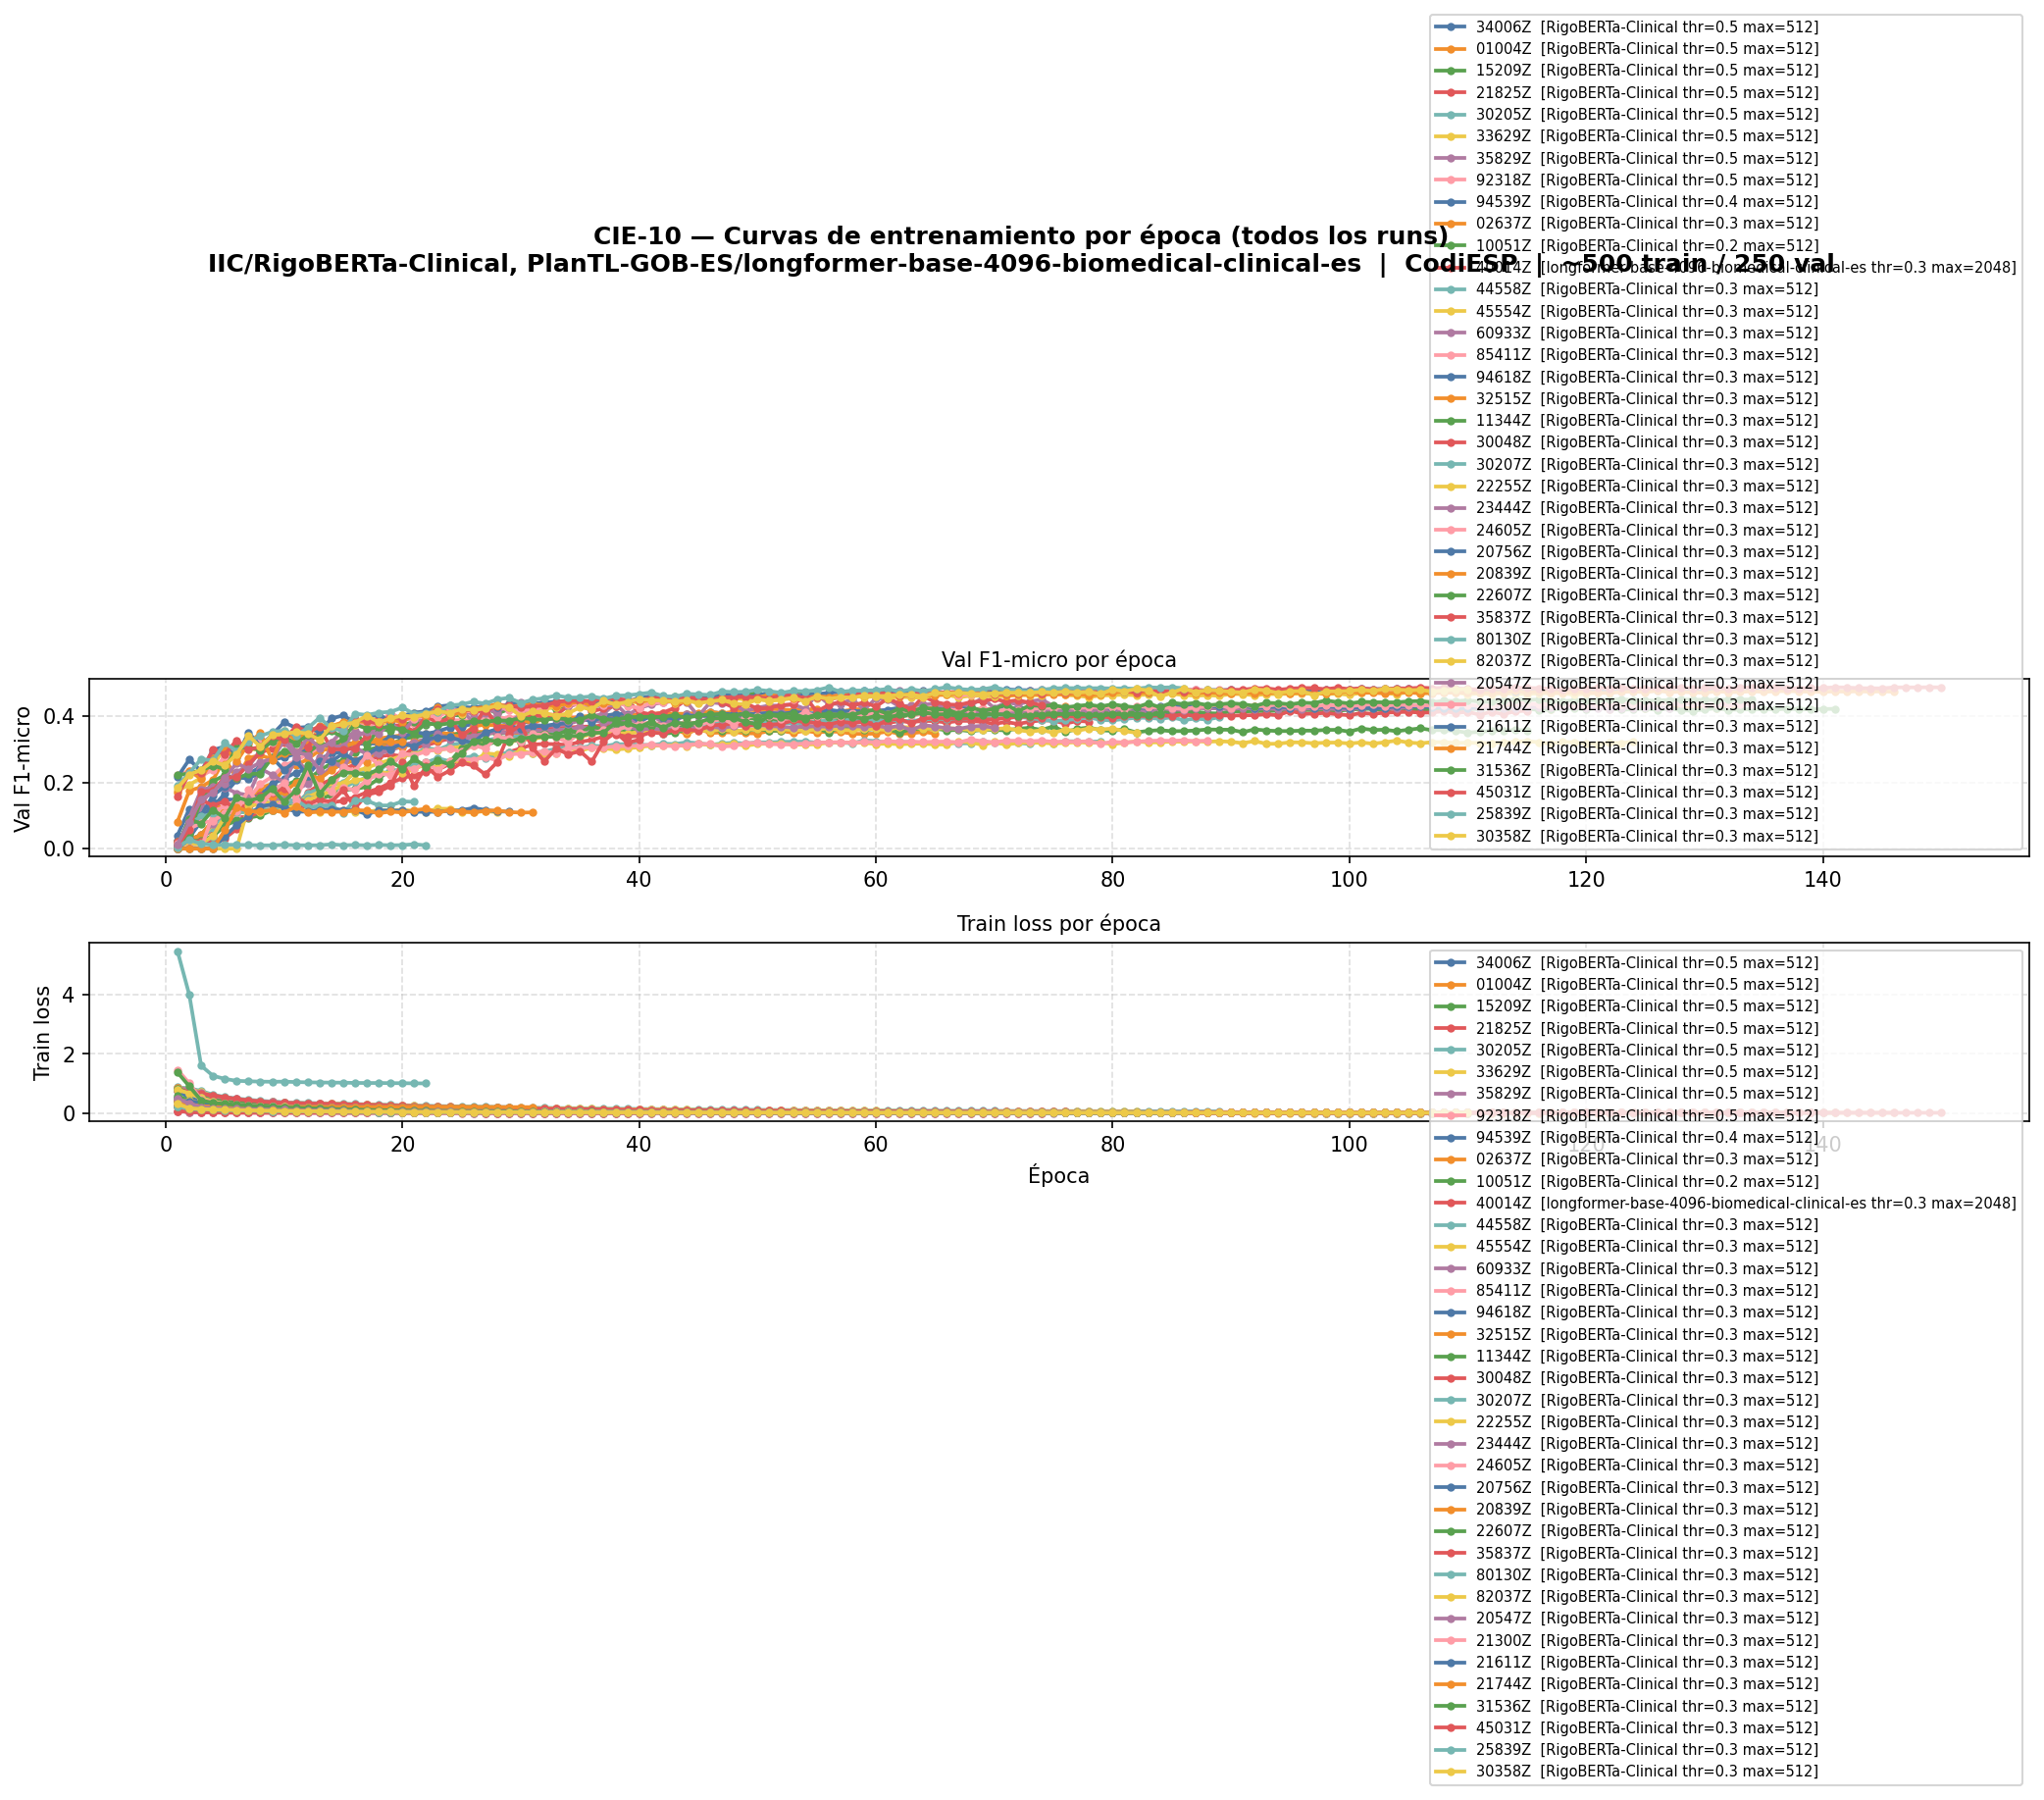
\includegraphics[width=\textwidth]{figs/all_epochs_graph}
\caption{Curvas de entrenamiento: F1-micro de validación y pérdida de entrenamiento por época.}
\label{fig:epochs-graph}
\end{figure}

\section{Artefactos del modelo}

Los artefactos del modelo desplegado en producción se encuentran en \texttt{ai\_engine/model/}:

\begin{description}
    \item[\texttt{classifier.pt}] Pesos del modelo PyTorch (ejecución del paso~36).
    \item[\texttt{thresholds.json}] Umbrales por clase optimizados sobre el conjunto de validación.
    \item[\texttt{config.json}] Metadatos del modelo activo: nombre, fichero de pesos, fichero de umbrales y parámetros de inferencia.
\end{description}
